% Options for packages loaded elsewhere
\PassOptionsToPackage{unicode}{hyperref}
\PassOptionsToPackage{hyphens}{url}
\PassOptionsToPackage{dvipsnames,svgnames,x11names}{xcolor}
\documentclass[
  ignorenonframetext,
]{beamer}
\newif\ifbibliography
\usepackage{pgfpages}
\setbeamertemplate{caption}[numbered]
\setbeamertemplate{caption label separator}{: }
\setbeamercolor{caption name}{fg=normal text.fg}
\beamertemplatenavigationsymbolsempty
% remove section numbering
\setbeamertemplate{part page}{
  \centering
  \begin{beamercolorbox}[sep=16pt,center]{part title}
    \usebeamerfont{part title}\insertpart\par
  \end{beamercolorbox}
}
\setbeamertemplate{section page}{
  \centering
  \begin{beamercolorbox}[sep=12pt,center]{section title}
    \usebeamerfont{section title}\insertsection\par
  \end{beamercolorbox}
}
\setbeamertemplate{subsection page}{
  \centering
  \begin{beamercolorbox}[sep=8pt,center]{subsection title}
    \usebeamerfont{subsection title}\insertsubsection\par
  \end{beamercolorbox}
}
% Prevent slide breaks in the middle of a paragraph
\widowpenalties 1 10000
\raggedbottom
\AtBeginPart{
  \frame{\partpage}
}
\AtBeginSection{
  \ifbibliography
  \else
    \frame{\sectionpage}
  \fi
}
\AtBeginSubsection{
  \frame{\subsectionpage}
}
\usepackage{iftex}
\ifPDFTeX
  \usepackage[T1]{fontenc}
  \usepackage[utf8]{inputenc}
  \usepackage{textcomp} % provide euro and other symbols
\else % if luatex or xetex
  \usepackage{unicode-math} % this also loads fontspec
  \defaultfontfeatures{Scale=MatchLowercase}
  \defaultfontfeatures[\rmfamily]{Ligatures=TeX,Scale=1}
\fi
\usepackage{lmodern}
\usefonttheme{serif} % use mainfont rather than sansfont for slide text
\ifPDFTeX\else
  % xetex/luatex font selection
  \ifLuaTeX
    \usepackage{luaotfload}
    \directlua{luaotfload.add_fallback("mainfontfallback",{
      "NotoColorEmoji:mode=harf"
    })}
  \fi
  \setmainfont[,RawFeature={fallback=mainfontfallback}]{NotoSans}
\fi
% Use upquote if available, for straight quotes in verbatim environments
\IfFileExists{upquote.sty}{\usepackage{upquote}}{}
\IfFileExists{microtype.sty}{% use microtype if available
  \usepackage[]{microtype}
  \UseMicrotypeSet[protrusion]{basicmath} % disable protrusion for tt fonts
}{}
\makeatletter
\@ifundefined{KOMAClassName}{% if non-KOMA class
  \IfFileExists{parskip.sty}{%
    \usepackage{parskip}
  }{% else
    \setlength{\parindent}{0pt}
    \setlength{\parskip}{6pt plus 2pt minus 1pt}}
}{% if KOMA class
  \KOMAoptions{parskip=half}}
\makeatother
\usepackage{longtable,booktabs,array}
\newcounter{none} % for unnumbered tables
\usepackage{calc} % for calculating minipage widths
\usepackage{caption}
% Make caption package work with longtable
\makeatletter
\def\fnum@table{\tablename~\thetable}
\makeatother
\usepackage{graphicx}
\makeatletter
\newsavebox\pandoc@box
\newcommand*\pandocbounded[1]{% scales image to fit in text height/width
  \sbox\pandoc@box{#1}%
  \Gscale@div\@tempa{\textheight}{\dimexpr\ht\pandoc@box+\dp\pandoc@box\relax}%
  \Gscale@div\@tempb{\linewidth}{\wd\pandoc@box}%
  \ifdim\@tempb\p@<\@tempa\p@\let\@tempa\@tempb\fi% select the smaller of both
  \ifdim\@tempa\p@<\p@\scalebox{\@tempa}{\usebox\pandoc@box}%
  \else\usebox{\pandoc@box}%
  \fi%
}
% Set default figure placement to htbp
\def\fps@figure{htbp}
\makeatother
\setlength{\emergencystretch}{3em} % prevent overfull lines
\providecommand{\tightlist}{%
  \setlength{\itemsep}{0pt}\setlength{\parskip}{0pt}}
\usetheme[sectionpage=none,numbering=fraction,progressbar=frametitle]{metropolis}
\usepackage{longtable,booktabs}
\usepackage{etoolbox}
\AtBeginEnvironment{longtable}{\tiny}
\AtBeginEnvironment{cslreferences}{\tiny}
\AtBeginEnvironment{Shaded}{\tiny}
\AtBeginEnvironment{verbatim}{\tiny}
\setmonofont[Contextuals={Alternate}]{FiraCodeNerdFontMono-Retina}
\usepackage{bookmark}
\IfFileExists{xurl.sty}{\usepackage{xurl}}{} % add URL line breaks if available
\urlstyle{same}
\hypersetup{
  pdftitle={Laboratórios de Sistemas e Serviços},
  pdfauthor={Mário Antunes},
  colorlinks=true,
  linkcolor={Maroon},
  filecolor={Maroon},
  citecolor={Blue},
  urlcolor={Blue},
  pdfcreator={LaTeX via pandoc}}

\title{\texorpdfstring{Laboratórios de Sistemas e
Serviços}{Laboratórios de Sistemas e Serviços}}
\author{\texorpdfstring{Mário Antunes}{Mário Antunes}}
\date{February 09, 2026}
\institute{Universidade de Aveiro}

\begin{document}
\frame{\titlepage}

\begin{frame}{Professors}
\protect\phantomsection\label{professors}
\begin{columns}[T]
\begin{column}{0.48\linewidth}
\begin{itemize}
\tightlist
\item
  \textbf{Name:} Mário Antunes
\item
  \textbf{E-Mail:}
  \href{mailto:mario.antunes@ua.pt}{\nolinkurl{mario.antunes@ua.pt}}
\item
  \textbf{Office:} 19.2.15 (IT1)
\end{itemize}
\end{column}

\begin{column}{0.48\linewidth}
\pandocbounded{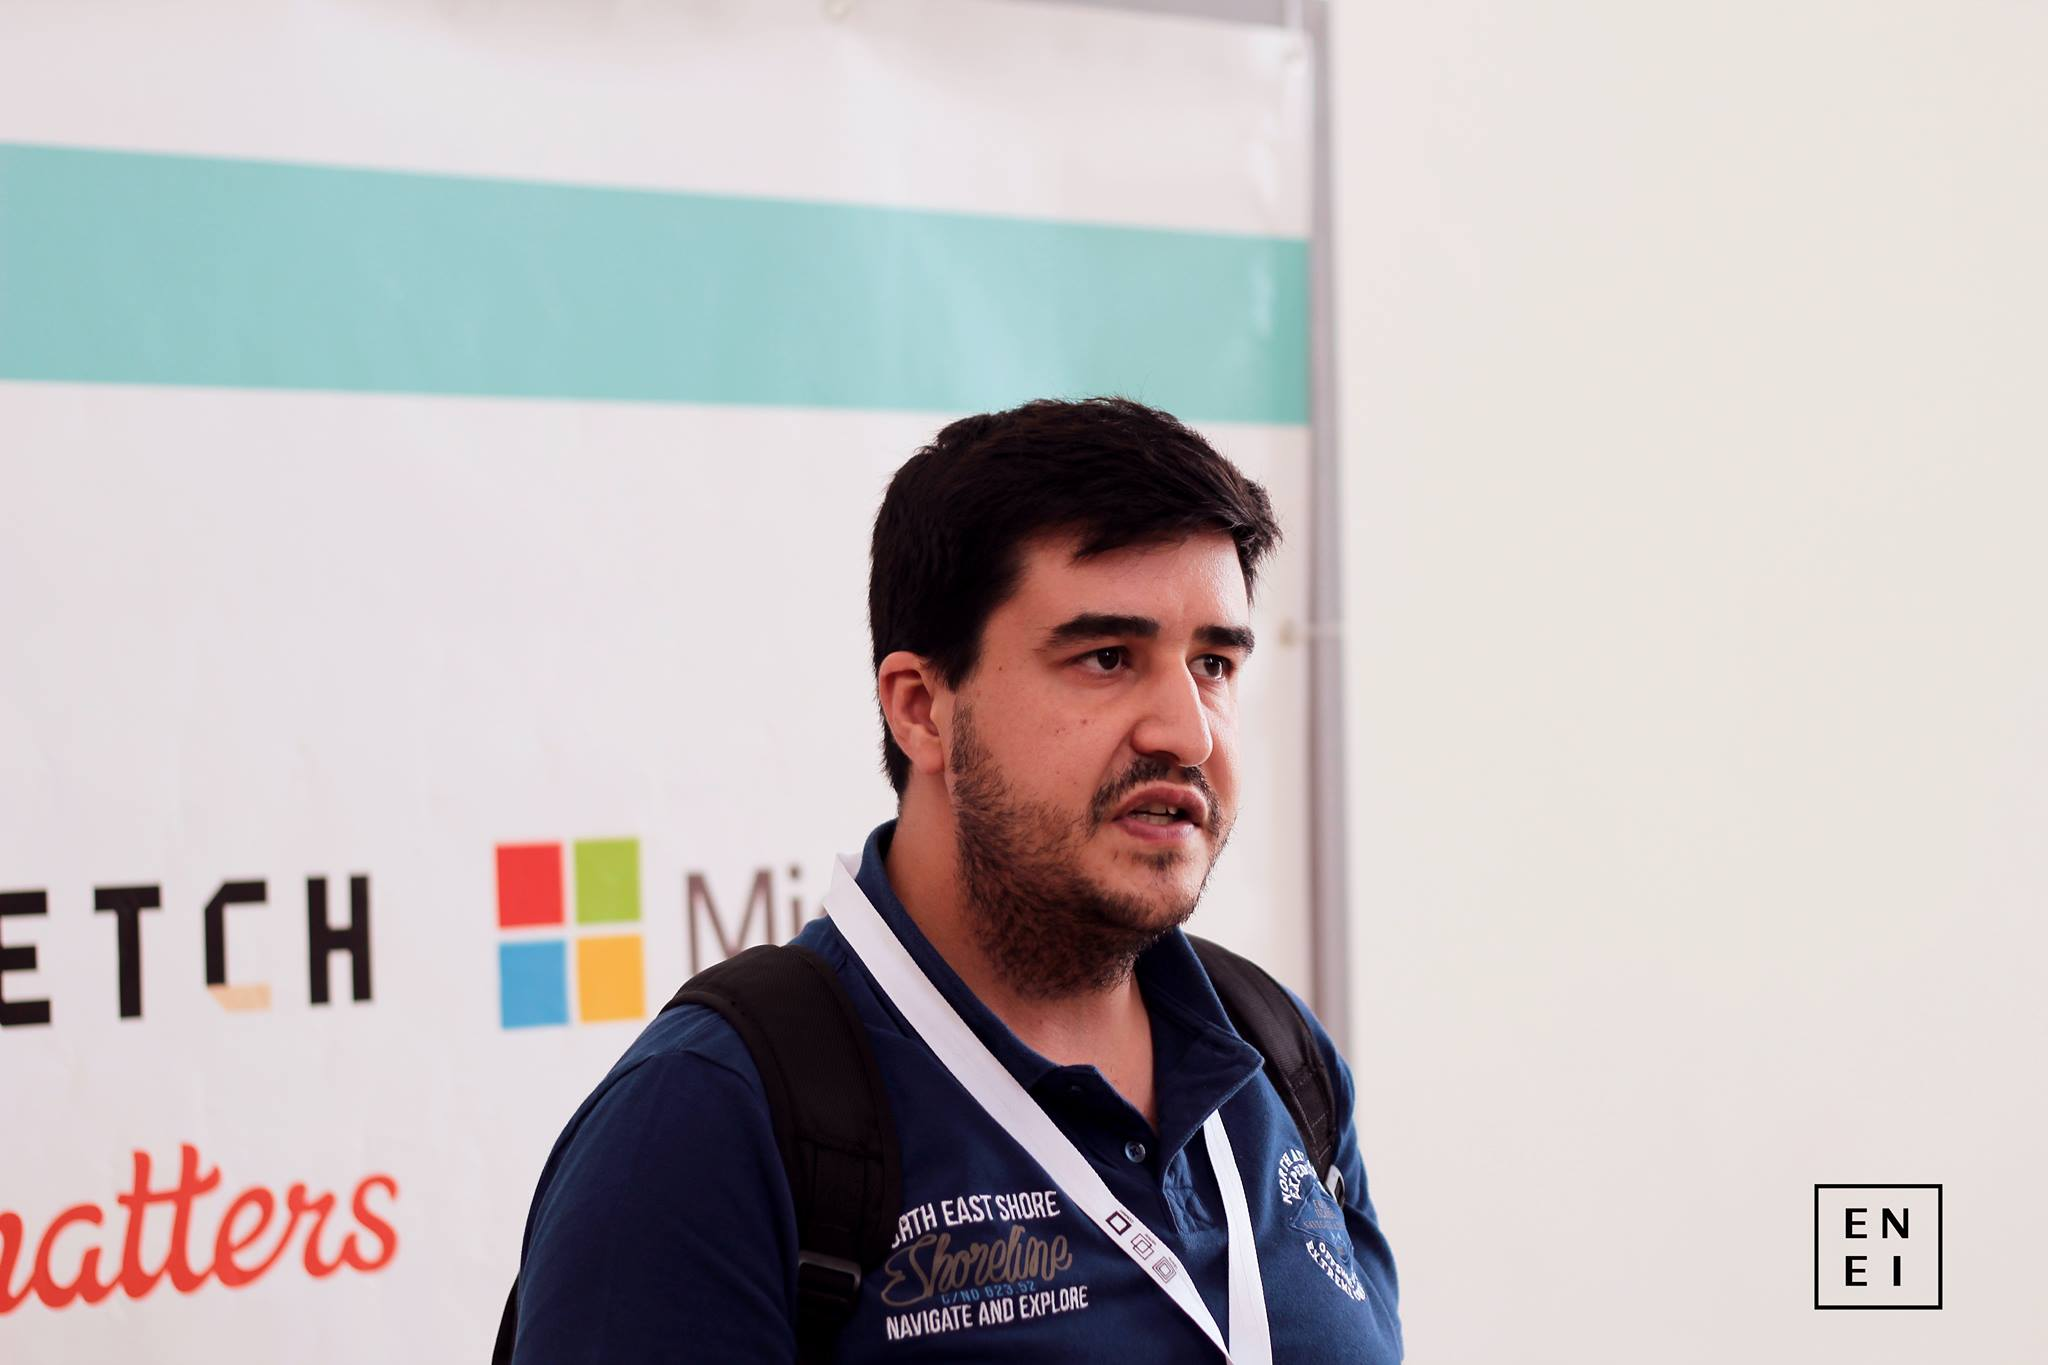
\includegraphics[keepaspectratio]{figures/mantunes.jpg}}
\end{column}
\end{columns}
\end{frame}

\begin{frame}{Professors}
\protect\phantomsection\label{professors-1}
\begin{columns}[T]
\begin{column}{0.48\linewidth}
\begin{itemize}
\tightlist
\item
  \textbf{Name:} Óscar Pereira
\item
  \textbf{E-Mail:} \href{mailto:omp@ua.pt}{\nolinkurl{omp@ua.pt}}
\item
  \textbf{Office:} 19.2.15 (IT1)
\end{itemize}
\end{column}

\begin{column}{0.48\linewidth}
\pandocbounded{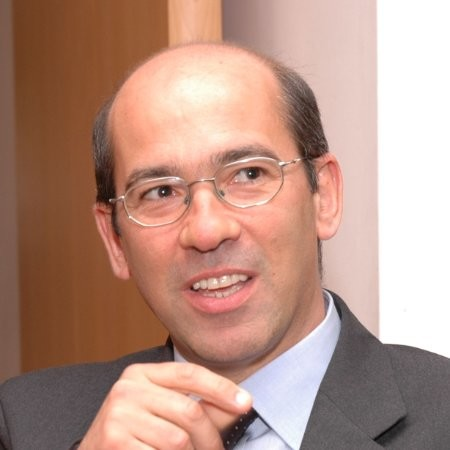
\includegraphics[keepaspectratio]{figures/omp.jpg}}
\end{column}
\end{columns}
\end{frame}

\begin{frame}{Class Introduction}
\protect\phantomsection\label{class-introduction}
Covering the following topics:

\begin{itemize}
\tightlist
\item
  C1. Virtualization and Containers
\item
  C2. WEB Servers
\item
  C3. Communication between Applications
\item
  C4. Communication in IP networks
\item
  C5. Representation and Communication of Digital Information
\item
  C6. Relational Databases and SQL
\end{itemize}
\end{frame}

\begin{frame}{Grading}
\protect\phantomsection\label{grading}
\begin{itemize}
\tightlist
\item
  50\% Theory + 50\% Practice
\item
  \emph{Discrete:} 25\% Project 1 + 25\% Project 2 + 50\% Exam
\item
  \emph{Final:} 50\% Final Exame + 50\% Project
\end{itemize}
\end{frame}

\begin{frame}{Class Schedule i}
\protect\phantomsection\label{class-schedule-i}
{\def\LTcaptype{none} % do not increment counter
\begin{longtable}[]{@{}lllll@{}}
\toprule\noalign{}
P1/P2 & P3/P5 & P4 & P6 & Topics \\
\midrule\noalign{}
\endhead
12-02-2026 & 10-02-2026 & 11-02-2026 & 09-02-2026 & C0 \\
19-02-2026 & 24-02-2026 & 18-02-2026 & 16-02-2026 & C0 \\
26-02-2026 & 03-03-2026 & 25-02-2026 & 23-02-2026 & C1 \\
05-03-2026 & 10-03-2026 & 04-03-2026 & 02-03-2026 & C1 \\
12-03-2026 & 17-03-2026 & 11-03-2026 & 09-03-2026 & C2 \\
19-03-2026 & 24-03-2026 & 18-03-2026 & 16-03-2026 & C2 \\
26-03-2026 & 31-03-2026 & 25-03-2026 & 23-03-2026 & C3 \\
\bottomrule\noalign{}
\end{longtable}
}
\end{frame}

\begin{frame}{Class Schedule ii}
\protect\phantomsection\label{class-schedule-ii}
{\def\LTcaptype{none} % do not increment counter
\begin{longtable}[]{@{}lllll@{}}
\toprule\noalign{}
P1/P2 & P3/P5 & P4 & P6 & Topics \\
\midrule\noalign{}
\endhead
16-04-2026 & 14-04-2026 & 15-04-2026 & 30-03-2026 & C4 \\
23-04-2026 & 21-04-2026 & 22-04-2026 & 13-04-2026 & C4 \\
07-05-2026 & 05-05-2026 & 06-05-2026 & 20-04-2026 & C5 \\
14-05-2026 & 12-05-2026 & 13-05-2026 & 04-05-2026 & C5 \\
21-05-2026 & 19-05-2026 & 20-05-2026 & 11-05-2026 & C6 \\
28-05-2026 & 26-05-2026 & 27-05-2026 & 18-05-2026 & C6 \\
& 02-06-2026 & 03-06-2026 & 25-05-2026 & Proj \\
& & & 01-06-2026 & Proj \\
\bottomrule\noalign{}
\end{longtable}
}
\end{frame}

\begin{frame}{Bibliography i}
\protect\phantomsection\label{bibliography-i}
\begin{itemize}
\tightlist
\item
  James F. Kurose and Keith W. Ross. 2021. Computer Networking: A
  Top-Down Approach (8th edition). Pearson.
\item
  Python Networking 101: Navigating essentials of networking, socket
  programming, AsyncIO, network testing, simulations and Ansible, Odette
  Windows, GiftforGits, 2023
\item
  Mailund, Thomas 2019 Introducing Markdown and Pandoc: Using Markup
  Language and Document Converter
\item
  William Shotts 2019 The Linux Command Line, 2nd Edition - A Complete
  Introduction
\end{itemize}
\end{frame}

\begin{frame}{Bibliography ii}
\protect\phantomsection\label{bibliography-ii}
\begin{itemize}
\tightlist
\item
  Paul McFedries 2023 HTML, CSS, \& JavaScript All-in-One For Dummies
\item
  Tanenbaum, A. S., \& Wetherall, D. J. (2011). \emph{Computer Networks}
  (5th Edition). Pearson.
\item
  Silberschatz, A., Korth, H. F., \& Sudarshan, S. (2019).
  \emph{Database System Concepts} (7th Edition). McGraw-Hill.
\item
  Kurose, J. F., \& Ross, K. W. (2021). \emph{Computer Networking: A
  Top-Down Approach} (8th Edition). Pearson.
\end{itemize}
\end{frame}

\end{document}
